\chapter{Changes That Cannot Be Undone}\label{ch:g5:irreversible-changes}

An egg is cracked into a hot pan. In a few seconds the clear, runny
white turns firm and white, and the yolk thickens. Take the pan off the
cooker, let the egg cool, put it in the fridge: it will never be a raw
egg again. Some changes can be undone and some cannot. Telling them apart
is the first step of chemistry.

\begin{recall}
A solid that \omterm{def:g2:mixing-and-dissolving:dissolve}{dissolves} in water is still there: when the water dries
away, the solid is left behind (\cref{ch:g2:mixing-and-dissolving}). A
\omterm{def:g4:what-a-fire-needs:burning}{burning} makes new substances --- ash, smoke, carbon dioxide, water
vapour --- and the \omterm{def:g4:what-a-fire-needs:fuel}{fuel} is gone for good (\cref{ch:g4:what-a-fire-needs}).
\end{recall}

\begin{omfigure}
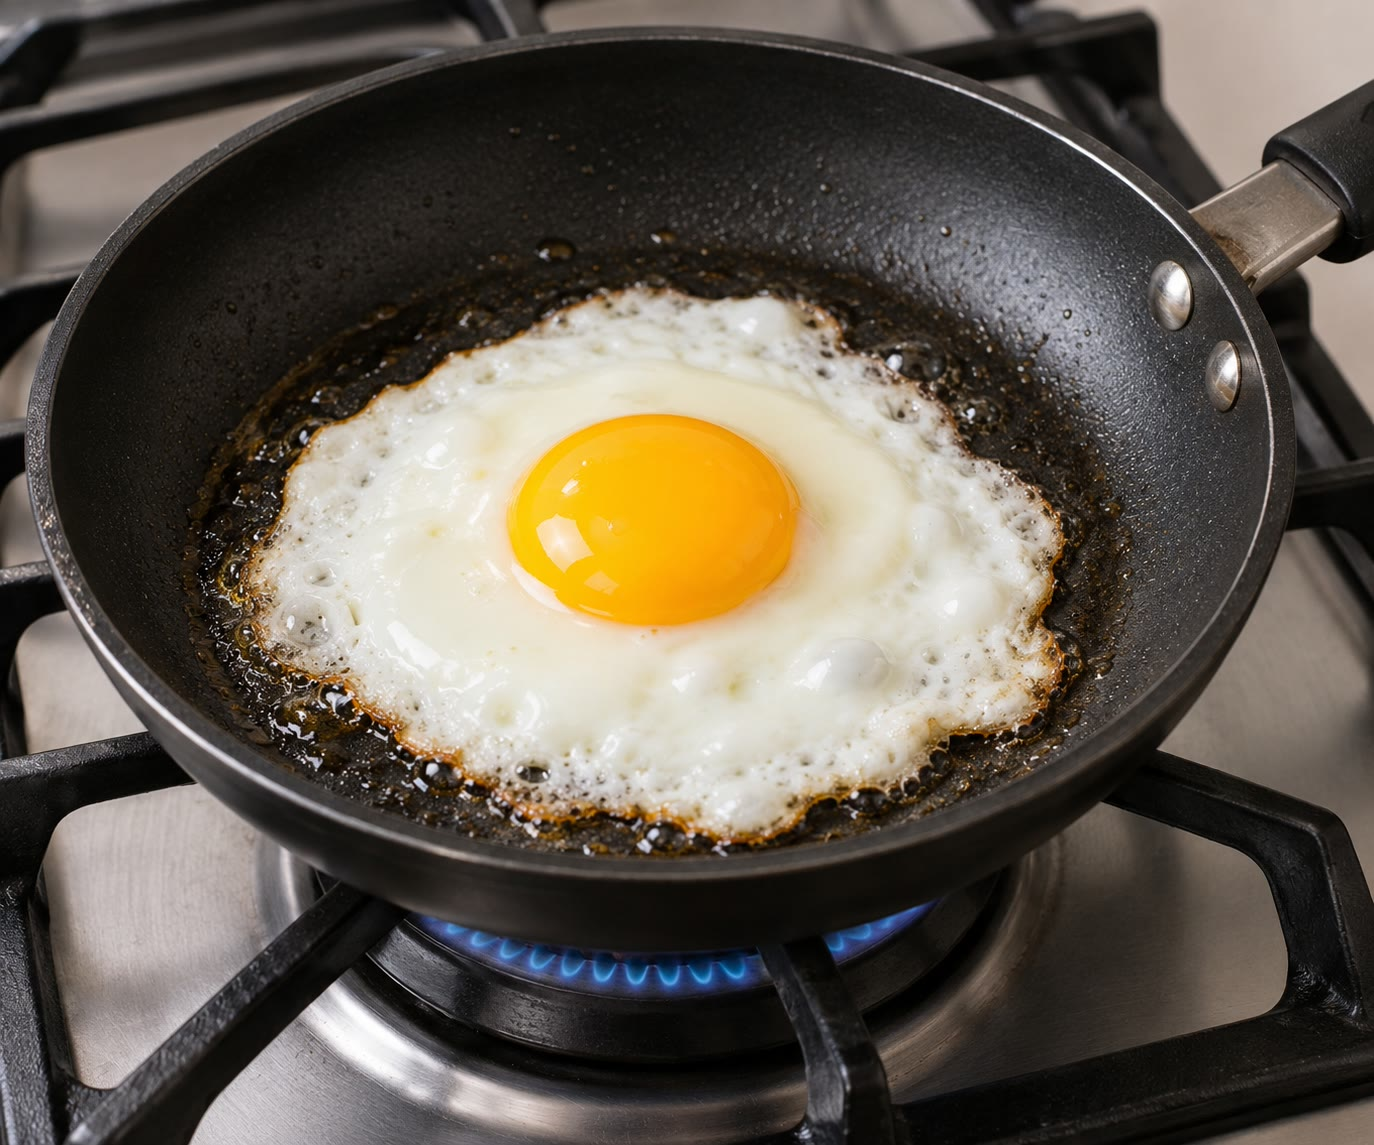
\includegraphics[width=0.55\linewidth]{images/book1/ai/g5-egg-frying.jpg}

{\small A frying egg: the clear white has turned firm and white, for
good.}
\end{omfigure}

\section{Changes that can be undone}

\begin{definition}[Reversible change]\label{def:g5:irreversible-changes:reversible}
A \emph{reversible change}\index{reversible change} is a change that can
be undone, so that we get back exactly what we started with.
\end{definition}

\begin{example}[Dissolving and drying]\label{ex:g5:irreversible-changes:dissolve}
Sugar stirred into water \omterm{def:g2:mixing-and-dissolving:dissolve}{dissolves}. Let the water evaporate, and the
sugar comes back: the same sugar, as sweet as before. Dissolving is a
\omterm{def:g5:irreversible-changes:reversible}{reversible change}.
\end{example}

\begin{example}[Ice and water]\label{ex:g5:irreversible-changes:ice}
An ice cube melts into water on a warm plate; put the water in the
freezer and it becomes ice again. Melting and freezing are \omterm{def:g5:irreversible-changes:reversible}{reversible
changes}. (Why water melts and freezes is told in the physics book.)
\end{example}

\begin{example}[Mixing]\label{ex:g5:irreversible-changes:mix}
Sand mixed with gravel can be sieved apart again; muddy water can be
filtered. Mixing is a \omterm{def:g5:irreversible-changes:reversible}{reversible change}: nothing new is made, and the
parts can be separated (\cref{ch:g3:separating-mixtures}).
\end{example}

\section{Changes that cannot be undone}

\begin{definition}[Irreversible change and chemical change]\label{def:g5:irreversible-changes:chemical-change}
An \emph{irreversible change}\index{irreversible change} is a change that
cannot simply be undone. Most of them are changes in which new
substances appear that were not there at the start: such a change is
called a \emph{chemical change}\index{chemical change}.
\end{definition}

\begin{example}[Six chemical changes]\label{ex:g5:irreversible-changes:six}
\begin{itemize}
  \item \textbf{Cooking an egg}: the runny, see-through white becomes
        firm and white.
  \item \textbf{Baking a cake}: a runny batter becomes a spongy cake,
        brown on the outside, with a new smell.
  \item \textbf{\omterm{def:g4:what-a-fire-needs:burning}{Burning}}: wood becomes ash, smoke, carbon dioxide and
        water vapour.
  \item \textbf{Rusting}: shiny iron left out in the rain becomes
        covered in a flaky orange-brown substance, rust.
  \item \textbf{Milk turning sour}: forgotten for days, milk thickens,
        forms lumps and smells sour.
  \item \textbf{A cut apple browning}: its pale flesh turns brown in the
        \omterm{def:g4:air-a-mixture-of-gases:air}{air} within an hour.
\end{itemize}
In each case something new has been made, and there is no simple way to
get back what we started with.
\end{example}

\begin{omfigure}
\begin{minipage}[t]{0.48\linewidth}\centering
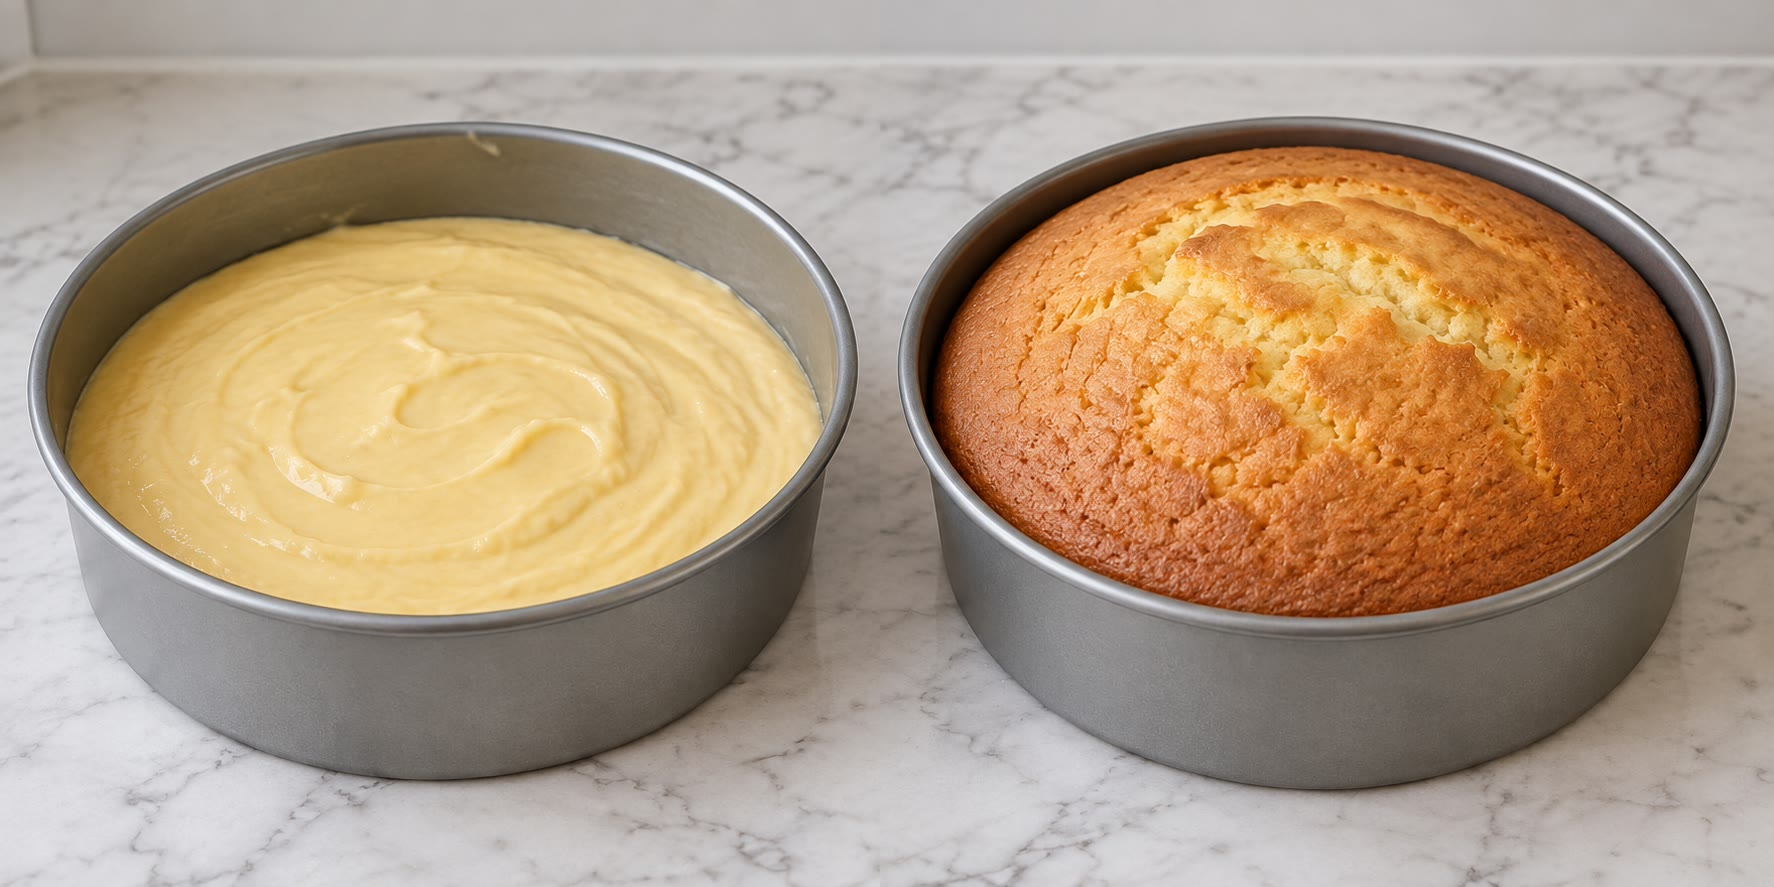
\includegraphics[width=\linewidth,height=4.6cm,keepaspectratio]{images/book1/ai/g5-cake-before-after.jpg}

{\small Batter before, cake after: baking cannot be undone.}
\end{minipage}\hfill
\begin{minipage}[t]{0.48\linewidth}\centering
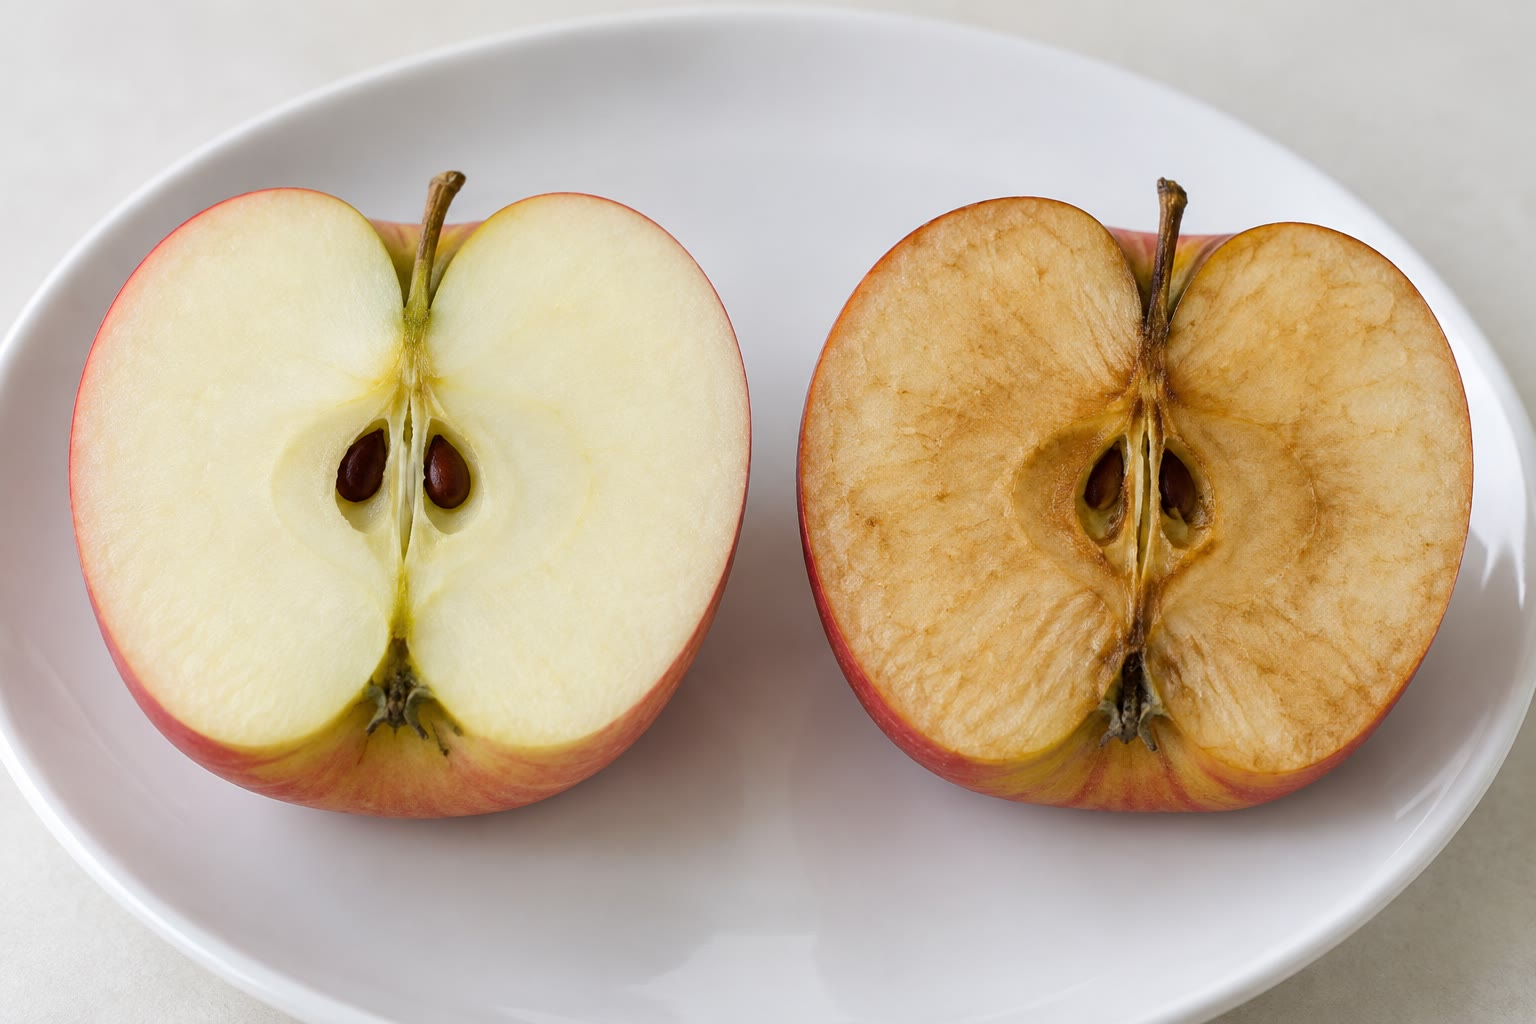
\includegraphics[width=\linewidth,height=4.6cm,keepaspectratio]{images/book1/ai/g5-apple-browning.jpg}

{\small A fresh half and a half left an hour in the \omterm{def:g4:air-a-mixture-of-gases:air}{air}.}
\end{minipage}
\end{omfigure}

\begin{omfigure}
\begin{tikzpicture}[font=\small]
  \node[font=\small\bfseries, omDef] at (2.7,4.6) {can be undone};
  \node[font=\small\bfseries, omProp] at (9.6,4.6) {cannot be undone};
  \draw[black!30] (6.1,4.9) -- (6.1,-0.3);
  % reversible pairs
  \foreach \y/\a/\b in {3.6/{sugar + water}/{sugar water}, 2.0/{ice}/{liquid water},
                        0.4/{sand + gravel}/{a mix}} {
    \node[draw=omDef, fill=omDef!6, rounded corners=2pt, minimum width=2.3cm,
      minimum height=0.8cm] at (0.9,\y) {\a};
    \node[draw=omDef, fill=omDef!6, rounded corners=2pt, minimum width=2.3cm,
      minimum height=0.8cm] at (4.6,\y) {\b};
    \draw[->, thick, omDef] (2.3,\y+0.12) -- (3.25,\y+0.12);
    \draw[<-, thick, omDef] (2.3,\y-0.12) -- (3.25,\y-0.12);
  }
  % irreversible ones
  \foreach \y/\a/\b in {3.6/{raw egg}/{cooked egg}, 2.0/{wood}/{ash, smoke, gases},
                        0.4/{iron}/{rust}} {
    \node[draw=omProp, fill=omProp!6, rounded corners=2pt, minimum width=2.0cm,
      minimum height=0.8cm] at (7.6,\y) {\a};
    \node[draw=omProp, fill=omProp!6, rounded corners=2pt, minimum width=2.9cm,
      minimum height=0.8cm] at (11.5,\y) {\b};
    \draw[->, thick, omProp] (8.8,\y) -- (9.85,\y);
  }
\end{tikzpicture}

{\small Left: \omterm{def:g5:irreversible-changes:reversible}{reversible changes}, the double arrow says they can go both
ways. Right: \omterm{def:g5:irreversible-changes:chemical-change}{chemical changes}, one way only.}
\end{omfigure}

\section{Clues that a new substance has appeared}

\begin{method}[Is it a chemical change? Look for the clues]\label{met:g5:irreversible-changes:clues}
A new substance is often given away by one of these clues:
\begin{enumerate}
  \item a new \textbf{colour} (the brown of a toasted slice of bread);
  \item \textbf{bubbles} of a gas appearing in a liquid without any
        heating (vinegar poured on baking soda);
  \item a new \textbf{smell} (sour milk, burnt toast);
  \item \textbf{heat or light} given out (a \omterm{def:g4:what-a-fire-needs:burning}{burning} candle);
  \item a \textbf{solid appearing} in a clear liquid, or lumps forming
        (milk curdling).
\end{enumerate}
One clue alone can mislead: boiling water bubbles, but nothing new is
made --- the bubbles are water vapour, and the water comes back when the
vapour cools. Look for several clues, and ask: can it be undone?
\end{method}

\begin{omfigure}
\begin{tikzpicture}[font=\small]
  \foreach \k/\t in {0/{new colour}, 1/{gas bubbles}, 2/{new smell},
                     3/{heat or light}, 4/{a solid appears}} {
    \begin{scope}[xshift=\k*3.2cm]
      \draw[omProp, line width=0.8pt, fill=omProp!5] (0,0) circle (1.0);
      \node[anchor=north, align=center] at (0,-1.15) {\t};
    \end{scope}
  }
  % 1: colour, a slice of toast half brown
  \fill[yellow!20, draw=brown!60] (-0.55,-0.5) rectangle (0.55,0.55);
  \fill[brown!55] (0,-0.5) rectangle (0.55,0.55);
  % 2: bubbles in a beaker
  \begin{scope}[xshift=3.2cm]
    \pic[transform shape, scale=0.45] at (0,-0.55) {beaker={0.7}{omWater!80}};
    \foreach \x/\y in {-0.15/-0.2,0.1/0.05,-0.05/0.25,0.18/-0.35,-0.2/0.15}
      \draw[black!55] (\x,\y) circle (0.05);
  \end{scope}
  % 3: smell, wavy lines
  \begin{scope}[xshift=6.4cm]
    \foreach \x in {-0.35,0,0.35} \draw[black!55, line width=0.8pt, decorate,
      decoration={snake, amplitude=1.5pt, segment length=6pt}] (\x,-0.6) -- (\x,0.6);
  \end{scope}
  % 4: a flame
  \begin{scope}[xshift=9.6cm]
    \fill[orange!80] (0,-0.6) .. controls (-0.45,-0.05) and (-0.15,0.35) .. (0,0.7)
      .. controls (0.15,0.35) and (0.45,-0.05) .. (0,-0.6);
    \fill[yellow!80] (0,-0.45) .. controls (-0.2,-0.1) and (-0.08,0.15) .. (0,0.3)
      .. controls (0.08,0.15) and (0.2,-0.1) .. (0,-0.45);
  \end{scope}
  % 5: solid settling in a test tube
  \begin{scope}[xshift=12.8cm]
    \pic[transform shape, scale=0.4] at (0,-0.65) {testtube={0.75}{omWater!80}};
    \fill[white, draw=black!40] (-0.08,-0.62) rectangle (0.08,-0.5);
    \foreach \x/\y in {-0.04/-0.3,0.04/-0.1,0/0.1} \fill[black!35] (\x,\y) circle (0.03);
  \end{scope}
\end{tikzpicture}

{\small Five clues that a \omterm{def:g5:irreversible-changes:chemical-change}{chemical change} may have happened.}
\end{omfigure}

\begin{inthelab}[Vinegar on baking soda]
The teacher puts a spoonful of baking soda, a white powder, at the
bottom of a beaker and pours in some vinegar. The mixture fizzes and
foams up at once: a gas is given off, a clue of a \omterm{def:g5:irreversible-changes:chemical-change}{chemical change}. When
the fizzing stops, the baking soda is gone and cannot be got back by
drying.
\end{inthelab}

\begin{omfigure}
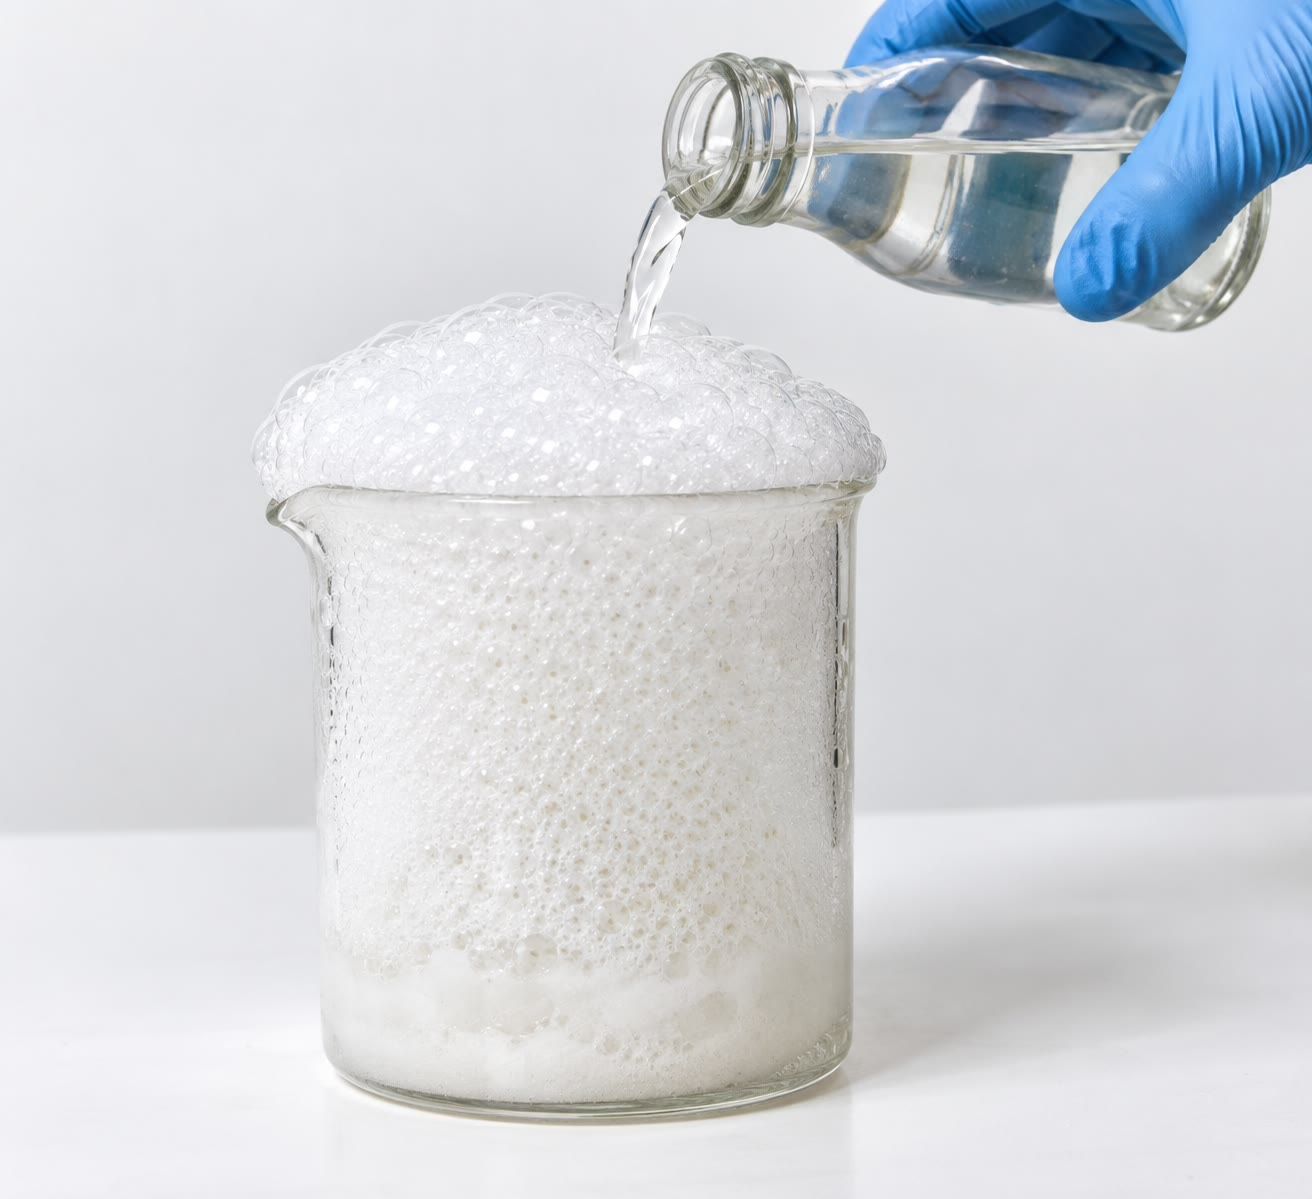
\includegraphics[width=0.5\linewidth]{images/book1/ai/g5-baking-soda-lab.jpg}

{\small Vinegar on baking soda: a gas is given off.}
\end{omfigure}

\section{Useful and harmful changes}

\begin{proposition}[Chemical changes around us]\label{prop:g5:irreversible-changes:around}
Many \omterm{def:g5:irreversible-changes:chemical-change}{chemical changes} are useful: cooking food, baking bread, \omterm{def:g4:what-a-fire-needs:burning}{burning}
gas to heat a home, plaster or cement setting hard. Others do damage:
iron rusting, food going off, wood rotting. We cannot undo them, but we
can slow them down:
\begin{itemize}
  \item food keeps longer in the cold of a fridge;
  \item paint or a film of oil keeps \omterm{def:g4:air-a-mixture-of-gases:air}{air} and water away from iron;
  \item a cut apple sprinkled with lemon juice browns more slowly.
\end{itemize}
\end{proposition}

\begin{omfigure}
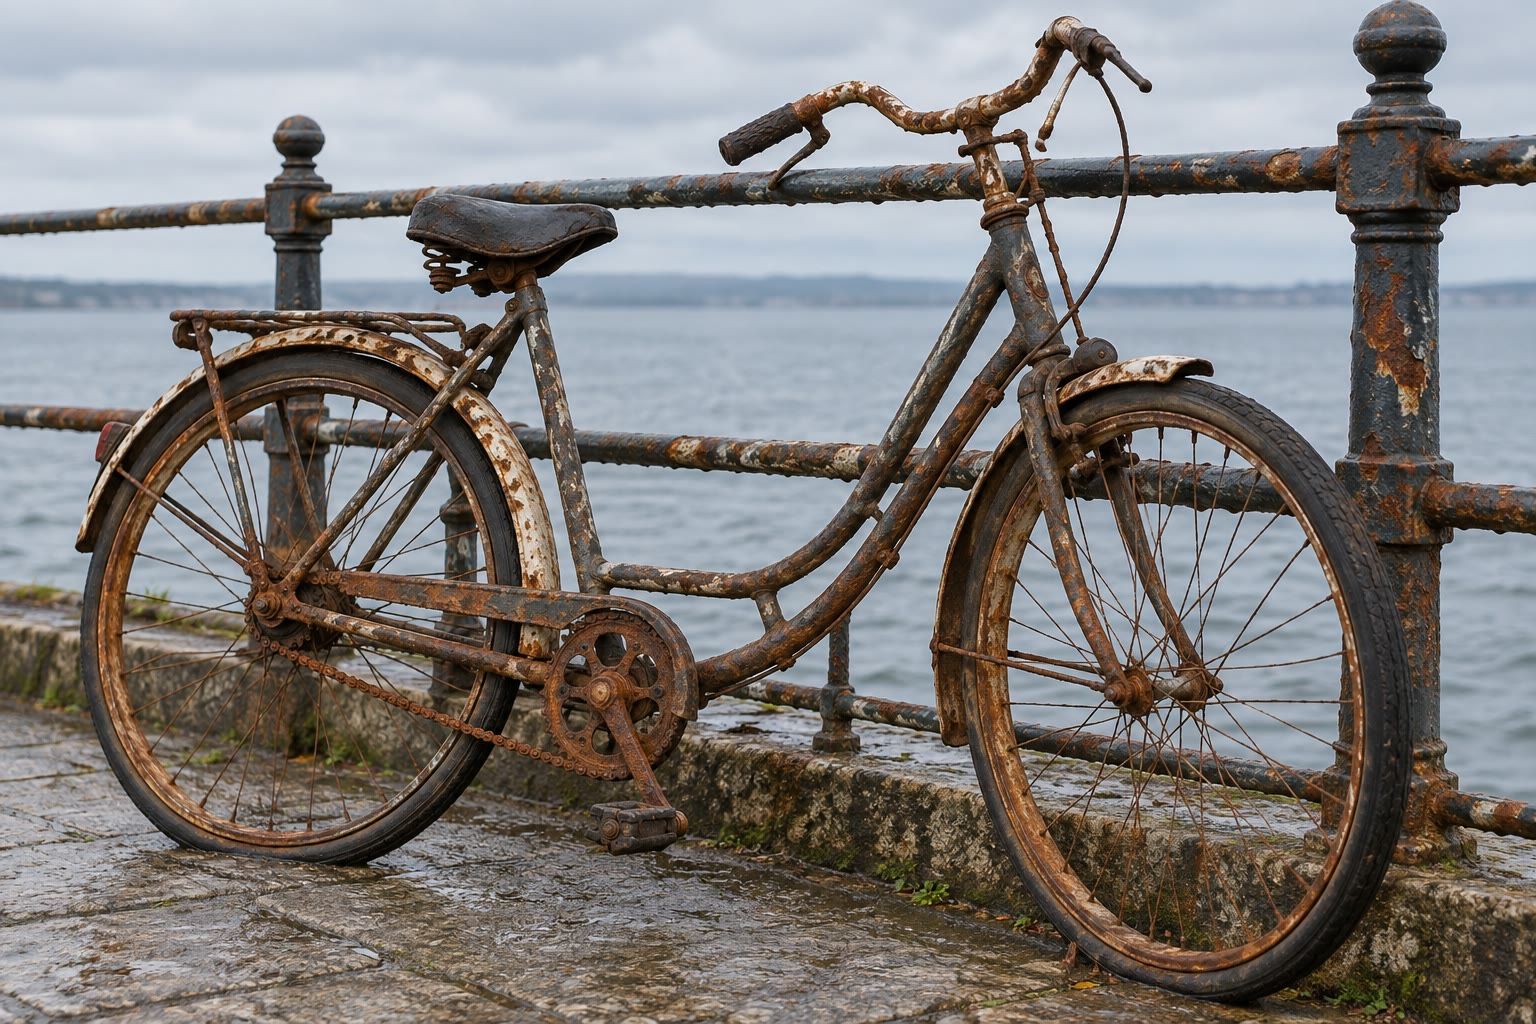
\includegraphics[width=0.55\linewidth]{images/book1/ai/g5-rusty-bicycle.jpg}

{\small A bicycle left out in the rain for years: the iron has rusted.}
\end{omfigure}

\begin{remark}[Undone, but not simply]\label{rem:g5:irreversible-changes:not-simply}
``Cannot be undone'' means that there is no simple way back, like
cooling or drying. Chemists can sometimes turn rust back into iron, but
only with a furnace and new substances: that is another \omterm{def:g5:irreversible-changes:chemical-change}{chemical
change}, not an undoing.
\end{remark}

\section{Exercises}

\begin{exercise}[$\star$]\label{exo:g5:irreversible-changes:1}
Say whether each change can be undone: melting chocolate, \omterm{def:g4:what-a-fire-needs:burning}{burning} a
match, dissolving salt in water, toasting bread.
\end{exercise}

\begin{exercise}[$\star$]\label{exo:g5:irreversible-changes:2}
What is a \omterm{def:g5:irreversible-changes:chemical-change}{chemical change}? Give two examples from the kitchen.
\end{exercise}

\begin{exercise}[$\star$]\label{exo:g5:irreversible-changes:3}
Salt is dissolved in water. How can the salt be got back? Is dissolving
a \omterm{def:g5:irreversible-changes:reversible}{reversible change}?
\end{exercise}

\begin{exercise}[$\star$]\label{exo:g5:irreversible-changes:4}
Which clue of a \omterm{def:g5:irreversible-changes:chemical-change}{chemical change} do you notice when milk turns sour?
Give two.
\end{exercise}

\begin{exercise}[$\star$]\label{exo:g5:irreversible-changes:5}
Look at the figure with two columns. Which changes have a double arrow?
What does the double arrow mean?
\end{exercise}

\begin{exercise}[$\star$]\label{exo:g5:irreversible-changes:6}
Why is a bicycle chain oiled? Which \omterm{def:g5:irreversible-changes:chemical-change}{chemical change} does the oil slow
down?
\end{exercise}

\begin{exercise}[$\star$]\label{exo:g5:irreversible-changes:7}
When vinegar is poured on baking soda, it fizzes. Which clue is this?
\end{exercise}

\begin{exercise}[$\star$]\label{exo:g5:irreversible-changes:8}
Name one useful \omterm{def:g5:irreversible-changes:chemical-change}{chemical change} and one harmful \omterm{def:g5:irreversible-changes:chemical-change}{chemical change}.
\end{exercise}

\begin{exercise}[$\star$]\label{exo:g5:irreversible-changes:9}
Why do we keep milk in the fridge?
\end{exercise}

\begin{exercise}[$\star\star$]\label{exo:g5:irreversible-changes:10}
Water bubbles when it boils. Is boiling a \omterm{def:g5:irreversible-changes:chemical-change}{chemical change}? Explain why a
single clue is not enough.
\end{exercise}

\begin{exercise}[$\star\star$]\label{exo:g5:irreversible-changes:11}
Tom says: ``When the candle burns, the wax just melts away, like ice.''
Use two clues to explain why \omterm{def:g4:what-a-fire-needs:burning}{burning} a candle is a \omterm{def:g5:irreversible-changes:chemical-change}{chemical change}, and
not only melting.
\end{exercise}
